
\begin{figure}
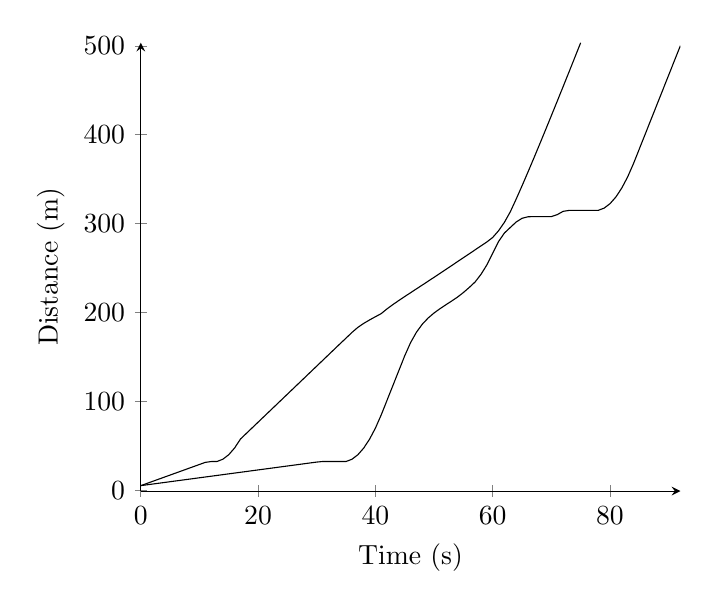
\begin{tikzpicture}
\begin{axis}[
legend style={anchor=west},
axis x line=bottom,
axis y line=left,
ymin=-1,
xlabel=Time (s),
ylabel=Distance (m),
]
\addplot[] coordinates {
(0, 5.1)
(1, 5.98407185106)
(2, 6.86814554278)
(3, 7.75222121159)
(4, 8.63629900791)
(5, 9.52037909795)
(6, 10.4044616659)
(7, 11.2885469163)
(8, 12.1726350774)
(9, 13.056726404)
(10, 13.9408211822)
(11, 14.8249197342)
(12, 15.7088375766)
(13, 16.5927594459)
(14, 17.4766857591)
(15, 18.3606640201)
(16, 19.2446484534)
(17, 20.1286397775)
(18, 21.0126388295)
(19, 21.8966465918)
(20, 22.7806642254)
(21, 23.6646931143)
(22, 24.5487349235)
(23, 25.4327916771)
(24, 26.3168658652)
(25, 27.2009605936)
(26, 28.0850797985)
(27, 28.9692285632)
(28, 29.8534136047)
(29, 30.7376440523)
(30, 31.6219327689)
(31, 32.2383371378)
(32, 32.2699168933)
(33, 32.2699168933)
(34, 32.2699168933)
(35, 32.2699168933)
(36, 34.7699168933)
(37, 39.7699168933)
(38, 47.2699168933)
(39, 57.2699168933)
(40, 69.7699168933)
(41, 84.7699168933)
(42, 101.369916893)
(43, 117.969916893)
(44, 134.569916893)
(45, 151.169916893)
(46, 165.992344434)
(47, 177.724584325)
(48, 186.763350745)
(49, 193.741438708)
(50, 199.339616093)
(51, 204.143655791)
(52, 208.548692901)
(53, 212.771257368)
(54, 217.238686427)
(55, 222.348003004)
(56, 228.078568356)
(57, 234.27113092)
(58, 242.801536775)
(59, 253.401316511)
(60, 266.501096246)
(61, 279.781298035)
(62, 289.351712276)
(63, 295.575076945)
(64, 301.721596781)
(65, 305.89436437)
(66, 307.605013212)
(67, 307.86435796)
(68, 307.86435796)
(69, 307.86435796)
(70, 307.86435796)
(71, 309.992534859)
(72, 313.715167306)
(73, 314.776186519)
(74, 314.869277834)
(75, 314.869277834)
(76, 314.869277834)
(77, 314.869277834)
(78, 314.869277834)
(79, 317.369277834)
(80, 322.369277834)
(81, 329.869277834)
(82, 339.869277834)
(83, 352.369277834)
(84, 367.369277834)
(85, 383.969277834)
(86, 400.569277834)
(87, 417.169277834)
(88, 433.769277834)
(89, 450.369277834)
(90, 466.969277834)
(91, 483.569277834)
(92, 500.169277834)
};
\addplot[] coordinates {
(0, 5.1)
(1, 7.48007836775)
(2, 9.86017128777)
(3, 12.2402820421)
(4, 14.6204149946)
(5, 17.0000834906)
(6, 19.3797842376)
(7, 21.759673408)
(8, 24.1396291121)
(9, 26.5196803008)
(10, 28.899876772)
(11, 31.2803141568)
(12, 32.1995792997)
(13, 32.269591524)
(14, 34.8396037483)
(15, 39.9096159726)
(16, 47.4796281969)
(17, 57.5496404212)
(18, 63.8592070264)
(19, 70.1691259843)
(20, 76.4794248112)
(21, 82.7901339669)
(22, 89.101287259)
(23, 95.4129223162)
(24, 101.725081144)
(25, 108.037810782)
(26, 114.351164078)
(27, 120.66520062)
(28, 126.979987841)
(29, 133.295602359)
(30, 139.612131594)
(31, 145.92967575)
(32, 152.248350234)
(33, 158.568288665)
(34, 164.889646616)
(35, 171.11260632)
(36, 177.436297617)
(37, 183.1296328)
(38, 187.621643042)
(39, 191.513499201)
(40, 195.147806556)
(41, 198.681139977)
(42, 204.087682254)
(43, 208.900502091)
(44, 213.42890366)
(45, 217.830436707)
(46, 222.177536371)
(47, 226.50183657)
(48, 230.816859217)
(49, 235.146907682)
(50, 239.504157444)
(51, 243.887037593)
(52, 248.289020478)
(53, 252.703601817)
(54, 257.12591216)
(55, 261.552782565)
(56, 265.982345649)
(57, 270.413631648)
(58, 274.846332582)
(59, 279.280998928)
(60, 284.349462811)
(61, 291.891197575)
(62, 301.411678297)
(63, 313.193142966)
(64, 327.474607635)
(65, 342.40328816)
(66, 357.729730335)
(67, 373.353497639)
(68, 389.202431071)
(69, 405.223342517)
(70, 421.376335707)
(71, 437.631124929)
(72, 453.964533121)
(73, 470.358727641)
(74, 486.869282453)
(75, 503.469282453)
};

\end{axis}
\end{tikzpicture}
\label{tik:distance:100:40}
\caption{100 percent diving with GSC on route $40$}
\end{figure}
